%
% $RCSfile$
%
% Copyright (c) 2002-2006. Christian Heller. All rights reserved.
%
% Permission is granted to copy, distribute and/or modify this document
% under the terms of the GNU Free Documentation License, Version 1.1 or
% any later version published by the Free Software Foundation; with no
% Invariant Sections, with no Front-Cover Texts and with no Back-Cover
% Texts. A copy of the license is included in the section entitled
% "GNU Free Documentation License".
%
% http://www.cybop.net
% - Cybernetics Oriented Programming -
%
% http://www.resmedicinae.org
% - Information in Medicine -
%
% Version: $Revision$ $Date$ $Author$
% Authors: Christian Heller <christian.heller@tuxtax.de>
%

\subsubsection{Pattern Simplification}
\label{pattern_simplification_heading}

The three communication patterns mentioned before had already been
reinvestigated for commonalities in \cite{hellerkunze}, which also embedded
them into the classical model of logical system layers (figure
\ref{simplification_figure}). For all kinds of communication, there is a:

\begin{itemize}
    \item[-] \emph{System} (Human User, Database, Remote Server)
    \item[-] \emph{Model} (View, ERM, DTO)
    \item[-] \emph{Translator} (Controller/ View Assembler, Data Mapper, DTO Assembler)
\end{itemize}

\begin{figure}[ht]
    \begin{center}
        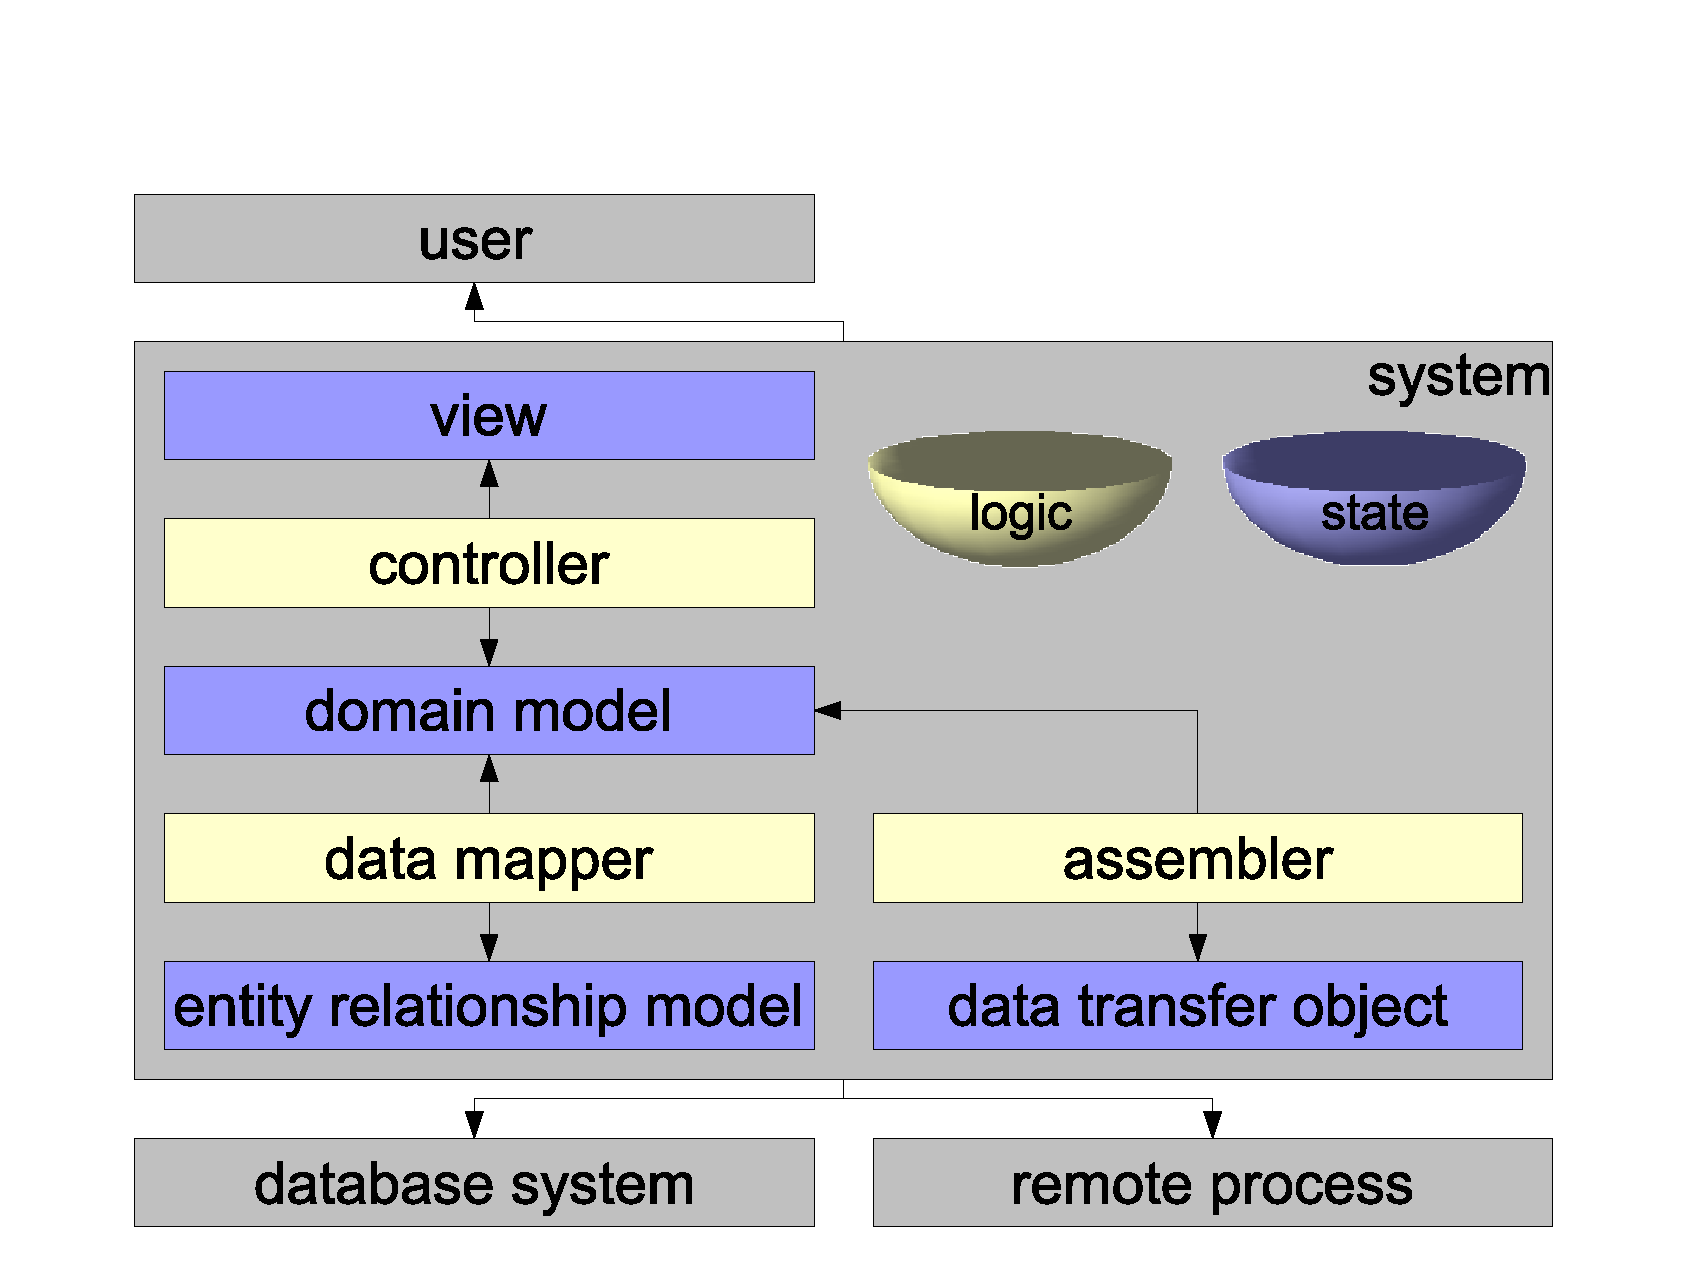
\includegraphics[scale=0.2]{vector/simplification.eps}
        \caption{Simplified Patterns in Layers}
        \label{simplification_figure}
    \end{center}
\end{figure}

All models represent certain states; all translators contain logic for
converting one state into another; all systems host their own, specific pool of
state- and logic knowledge. Realising this, a much clearer view on software
architectures can be retrieved.

Because domain models differ between systems, each system needs its own
translator models. Only communication models need to be agreed upon between
systems; they need to be understood by both communication partners.
